%==============================================================================
%  Invariance vs robustness  --  TUM-themed talk deck (serious academic rebuild)
%  Grounded in: the papers (read end to end), the praktikum report + repo, the code,
%  a style guide distilled from 6 real ICML/NeurIPS/ICLR decks, and a novelty audit.
%  Speaker notes via \note{} (enable with \setbeameroption{show notes}).
%  TUM logo: assets/tum_logo.pdf.
%==============================================================================
\documentclass[aspectratio=169,10pt]{beamer}
\usepackage[T1]{fontenc}
\usepackage[utf8]{inputenc}
\usepackage{lmodern}
\usepackage{amsmath,amssymb,amsfonts}
\usepackage{graphicx}
\usepackage{booktabs}
\usepackage{tikz}
\usepackage{pifont}
\usetikzlibrary{arrows.meta,positioning,calc,decorations.pathreplacing}

%------------------------------------------------------------------ TUM palette
\definecolor{TUMblue}{HTML}{0065BD}
\definecolor{TUMdark}{HTML}{005293}
\definecolor{TUMdarker}{HTML}{003359}
\definecolor{TUMorange}{HTML}{E37222}
\definecolor{ink}{HTML}{1F2933}
\definecolor{slate}{HTML}{52606D}
\definecolor{good}{HTML}{2F855A}
\definecolor{bad}{HTML}{9B2C2C}
\definecolor{paper}{HTML}{FFFFFF}

\usetheme{default}
\setbeamercolor{normal text}{fg=ink,bg=paper}
\setbeamercolor{structure}{fg=TUMblue}
\setbeamercolor{frametitle}{fg=TUMdarker,bg=paper}
\setbeamercolor{itemize item}{fg=TUMblue}
\setbeamercolor{itemize subitem}{fg=slate}
\setbeamercolor{block title}{fg=paper,bg=TUMblue}
\setbeamercolor{block body}{fg=ink,bg=TUMblue!7}
\setbeamercolor{block title alerted}{fg=paper,bg=TUMdarker}
\setbeamercolor{block body alerted}{fg=ink,bg=TUMdarker!7}
\setbeamerfont{frametitle}{series=\bfseries,size=\large}
\setbeamerfont{title}{series=\bfseries,size=\huge}
\setbeamertemplate{navigation symbols}{}
\setbeamertemplate{itemize item}{\small\raise0.15ex\hbox{\textbullet}}
\setbeamertemplate{itemize subitem}{\footnotesize\raise0.1ex\hbox{--}}
\setbeamertemplate{blocks}[rounded][shadow=false]
\setbeamertemplate{theorems}[numbered]
\newtheorem{proposition}{Proposition}

\newcommand{\tumlogo}{%
  \IfFileExists{assets/tum_logo.pdf}{
\includegraphics[height=0.9cm]{assets/tum_logo.pdf}}%
  {\colorbox{TUMblue}{\textcolor{white}{\bfseries\,TUM\,}}}}

\setbeamertemplate{frametitle}{%
  \vspace{0.5em}%
  \begin{beamercolorbox}[wd=\paperwidth,leftskip=0.9em,rightskip=0.9em]{frametitle}%
    \usebeamerfont{frametitle}\insertframetitle%
    \ifx\insertframesubtitle\empty\else
      \\[0.1em]{\small\normalfont\color{slate}\insertframesubtitle}%
    \fi
    \vspace{0.1em}{\color{TUMblue}\hrule height 1.4pt}%
  \end{beamercolorbox}}
\setbeamertemplate{footline}{%
  \hbox{\begin{beamercolorbox}[wd=\paperwidth,ht=2.2ex,dp=1ex,leftskip=0.9em,rightskip=0.9em]{}%
    {\color{slate}\scriptsize Invariance vs robustness
    \hfill Technical University of Munich\hfill \insertframenumber}%
  \end{beamercolorbox}}}

\newcommand{\etaL}{\ensuremath{\eta/L}}
\newcommand{\tb}[1]{{\color{TUMblue}#1}}
\newcommand{\key}[1]{{\color{TUMdarker}\bfseries #1}}
\newcommand{\good}[1]{{\color{good}#1}}
\newcommand{\bad}[1]{{\color{bad}#1}}
\newcommand{\cok}{\textcolor{good}{\ding{51}}}
\newcommand{\cno}{\textcolor{bad}{\ding{55}}}

\title{Invariance vs robustness}
\author{Anass Al Ammiri}
\institute{Technical University of Munich}
\date{}

\begin{document}

%========================= TITLE ==============================================
{\setbeamertemplate{footline}{}
\begin{frame}[plain]
  \vspace{0.4em}\begin{flushright}\tumlogo\end{flushright}\vspace{0.6em}
  \vspace{1.2em}
  \begin{center}
    {\usebeamerfont{title}\color{TUMdarker} Invariance vs robustness}\\[0.6em]
    {\large\color{TUMblue} What orders a model's adversarial robustness}\\[1.4em]
    {\color{TUMblue}\rule{0.42\textwidth}{1.2pt}}
  \end{center}
  \vfill
  \begin{center}\small\color{slate}
    A project growing out of the practical course on adversarial robustness and shift invariance.
    Prior work relates the two and reaches opposite conclusions; we build a margin-based diagnostic and
    test what tells them apart, from small classifiers to foundation-model encoders.
  \end{center}
  \note{Say: this is a project that grew out of the practical course. It is about two properties of a
  vision model, invariance and adversarial robustness. The literature has related them and reached
  opposite conclusions. I will show what actually orders robustness, and it is not the invariance metric
  people track.}
\end{frame}}

%========================= MOTIVATION =========================================
\begin{frame}{The two properties, on one image}{}
  \vspace{0.1em}
  \begin{center}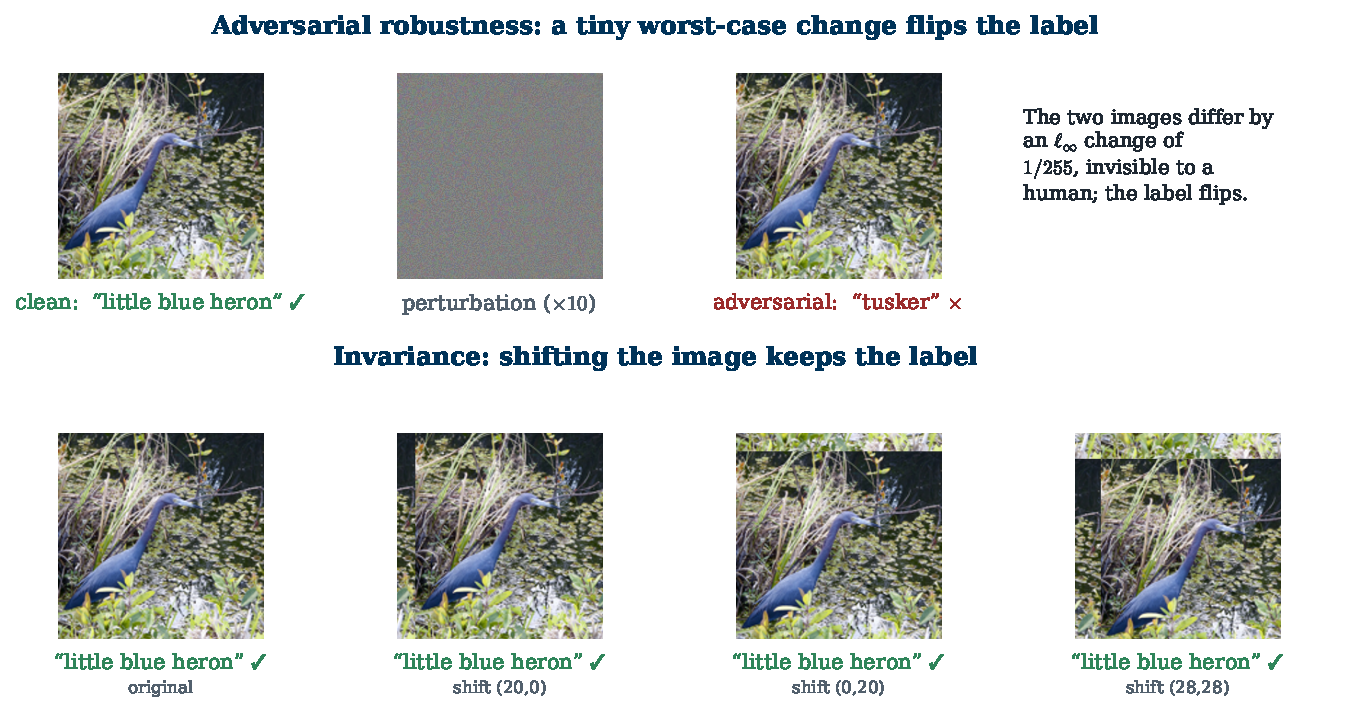
\includegraphics[width=0.74\linewidth]{figures/concept_imagenet.pdf}\end{center}
  \vspace{0.1em}
  {\scriptsize\color{slate} A real image and an ImageNet classifier. An $\ell_\infty$ change of $1/255$,
  invisible to a person, changes the label (top). Shifting the image does not (bottom).}
  \note{Say: here is one image and a standard classifier. On top, a change of one part in 255, which you
  cannot see, turns a heron into an elephant. On the bottom, sliding the image around does nothing to the
  label. Robustness is about the top row; invariance is about the bottom row. The question is how they
  relate.}
\end{frame}

%========================= THE QUESTION =======================================
\begin{frame}{The literature relates them, and disagrees}{}
  \vspace{0.2em}
  \begin{columns}[T]
    \begin{column}{0.49\textwidth}
      {\footnotesize\textbf{\color{good}Invariance helps}}
      \begin{itemize}\scriptsize\itemsep3pt
        \item \tb{Zhang, ICML 2019.} Anti-aliased pooling raises shift-consistency and corruption robustness.
        \item \tb{Saha \& Gokhale, WACV 2024.} ``Better shift invariance is generally correlated with
          better adversarial robustness'' ($\S6.4$); PGD/FGSM, one ResNet-34.
        \item \tb{Grabinski et al., 2023.} Alias-free downsampling improves robustness; FGSM/PGD/APGD.
        \item \tb{Wang et al., 2025.} Equivariant CNNs improve robustness on CIFAR; FGSM and PGD.
      \end{itemize}
    \end{column}
    \begin{column}{0.49\textwidth}
      {\footnotesize\textbf{\color{bad}Invariance hurts, or trades off}}
      \begin{itemize}\scriptsize\itemsep3pt
        \item \tb{Ge et al., NeurIPS 2021.} A shift-invariant linear classifier uses only the input
          average; the margin drops from $2$ to $2/\sqrt d$. PGD on MNIST/Fashion.
        \item \tb{Kamath et al., NeurIPS 2021.} A proven trade-off between spatial and adversarial
          robustness; their rate of invariance is our consistency; rotation as a cyclic shift.
      \end{itemize}
      \vspace{0.5em}
      {\scriptsize\color{slate} These lines use different data, models, and attacks. None on the left
      uses a parameter-free strong attack. Ge's own reading: invariance hurts only when it both raises
      the dimension and shrinks the margin.}
    \end{column}
  \end{columns}
  \note{Say: one line of work, anti-aliasing and equivariance, reports that invariance helps robustness.
  Another, Ge and Kamath, reports the opposite or a trade-off. They study different settings, and,
  importantly, the ``helps'' side only ever used gradient attacks like FGSM and PGD, never a strong
  parameter-free attack. So the disagreement is not resolved. My question is: what quantity actually
  orders robustness across models?}
\end{frame}

%========================= SCOPE / OUTLINE ====================================
\begin{frame}{How we frame the project}{}
  \vspace{0.4em}
  \begin{columns}[T]
    \begin{column}{0.5\textwidth}
      {\footnotesize\textbf{What the project does}}
      \begin{itemize}\footnotesize\itemsep3pt
        \item defines a margin-to-sensitivity ratio and proves when it brackets the robust radius;
        \item shows shift-consistency does not order robustness and this ratio does, across model families;
        \item shows the ``invariance helps'' effect is a weak-attack artifact;
        \item adds the gradient's shape to rank already-robust models.
      \end{itemize}
    \end{column}
    \begin{column}{0.5\textwidth}
      {\footnotesize\textbf{What it does not claim}}
      \begin{itemize}\footnotesize\itemsep3pt
        \item that the ratio is a new object; it is a Lipschitz--margin certificate we refine;
        \item co-existence of invariance and robustness as a discovery;
        \item a new attack or a new defense; the ratio is a diagnostic.
      \end{itemize}
    \end{column}
  \end{columns}
  \vspace{0.4em}
  {\footnotesize\color{slate} Structure: (1) where the project started; (2) the ratio and its theory;
  (3) experiments; (4) ranking robust models; (5) limitations and questions.}
  \note{Say: to frame the project. It proves a bracket, shows a dissociation across families, debunks the
  weak-attack effect, and adds a shape term for ranking. It does not claim the ratio is new, does not
  claim co-existence as a discovery, and does not propose an attack or a defense.}
\end{frame}

%========================= PRAKTIKUM ==========================================
\begin{frame}{Where this started}{A recap of the practical course, in two points}
  \vspace{0.3em}
  \begin{itemize}\footnotesize\itemsep7pt
    \item \key{What we did: reproduce and extend Ge et al.\ on MNIST and Fashion-MNIST.}
      \begin{itemize}\scriptsize\itemsep2pt
        \item Reproduced their ordering with FGSM and PGD ($\ell_2$, $\ell_\infty$): more shift-consistency
          went with lower robust accuracy across their models.
        \item Extended it to standard architecture choices, pooling type, kernel size, depth, an added
          dense layer, measuring robust accuracy and shift-consistency for each.
      \end{itemize}
    \item \key{What we found, and what it left open.}
      \begin{itemize}\scriptsize\itemsep2pt
        \item The simple ``more consistency, less robust'' ordering broke: several CNNs were both
          shift-consistent and as robust as the fully-connected baseline. We used a
          consistency-versus-robustness graph to screen architectures.
        \item It did not say which quantity predicts robustness when consistency does not, and it used
          only weak attacks. That is what the rest of the project addresses.
      \end{itemize}
  \end{itemize}
  \note{Say: this began as a course project I did with Maha. We reproduced Ge with FGSM and PGD, then
  tested the standard architecture knobs. We found the simple ordering was not always right: some CNNs
  were both consistent and robust. We proposed screening models on a consistency-robustness graph. But
  two things were unfinished: which quantity predicts robustness, and whether the effect survives a
  strong attack. That is what the rest of the talk addresses.}
\end{frame}

%========================= BRIDGE =============================================
\begin{frame}{From the project to now}{Recent papers, and what is still open}
  \vspace{0.5em}
  \begin{itemize}\footnotesize\itemsep7pt
    \item \key{The co-existence we saw is now in a published paper.} During the practical course we found
      that invariance and robustness can co-exist. TIPS \tb{(Saha \& Gokhale, 2024)} later reported the
      same correlation, so this observation is now established in the literature.
    \item \key{There are still additions we can make on top of it.} A parameter-free strong attack was
      never applied to this line; the invariance metric was never tested for whether it \emph{orders}
      robustness; and there is no quantity that predicts robustness without an attack.
    \item \key{The question.} Is there a quantity, computable without an attack, that orders adversarial
      robustness across models, where shift-consistency does not?
  \end{itemize}
  \note{Say: three things pushed the project forward. First, the co-existence we saw in the course is now
  in a published paper, TIPS from 2024, so it is established. Second, there are still additions we can
  make on top of it: nobody ran a strong parameter-free attack, nobody checked whether the invariance
  metric actually orders robustness, and there was no attack-free predictor. Third, that is the question:
  is there such a quantity? The answer is yes, and it is a margin quantity.}
\end{frame}

%========================= SETUP: WHY DIFFERENT ===============================
\begin{frame}{Invariance and robustness are different directions}{}
  \vspace{0.2em}
  \begin{columns}[T]
    \begin{column}{0.46\textwidth}
      \centering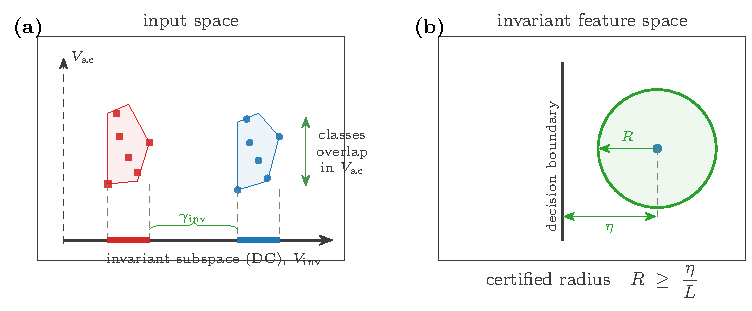
\includegraphics[width=0.99\linewidth]{figures/concept.pdf}\\[0.3em]
      {\scriptsize\color{slate} Imposing invariance projects the classes onto the invariant part
      (their average); robustness is the distance $R\ge\etaL$ to the boundary.}
    \end{column}
    \begin{column}{0.5\textwidth}
      \centering
      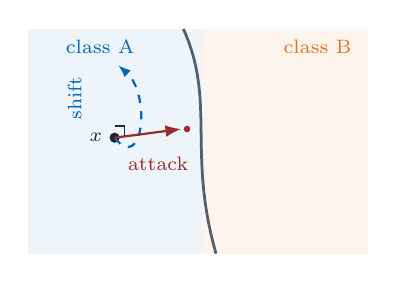
\begin{tikzpicture}[scale=0.92,every node/.style={font=\scriptsize}]
        \fill[TUMblue!7] (-0.1,-0.1) rectangle (2.3,3.0);
        \fill[TUMorange!8] (2.3,-0.1) rectangle (4.6,3.0);
        \draw[slate,line width=1pt] (2.5,-0.1) .. controls (2.1,1.3) and (2.5,2.0) .. (2.05,3.0);
        \node[TUMblue] at (0.9,2.75){class A}; \node[TUMorange] at (3.9,2.75){class B};
        \fill[ink] (1.1,1.5) circle (2pt); \node[ink,left=1pt] at (1.1,1.5){$x$};
        % shift: walks parallel to boundary (around it)
        \draw[TUMblue,thick,dashed,-{Latex[length=1.6mm]}] (1.1,1.5) .. controls (1.5,1.0) and (1.6,2.1) .. (1.15,2.5);
        \node[TUMblue] at (0.55,2.05){\rotatebox{90}{shift}};
        % adversarial: walks toward the boundary (crosses)
        \draw[bad,thick,-{Latex[length=2mm]}] (1.1,1.5)--(2.02,1.62);
        \node[bad,below=1pt] at (1.7,1.4){attack};
        \fill[bad] (2.1,1.62) circle (1.3pt);
        \draw[ink,line width=0.5pt] (1.1,1.66)--(1.24,1.66)--(1.24,1.52);
      \end{tikzpicture}\\[0.3em]
      {\scriptsize\color{slate} The shift walks \emph{around} the boundary (label kept); the attack walks
      \emph{toward} it (label crossed). Near-orthogonal directions.}
    \end{column}
  \end{columns}
  \note{Say: geometrically these are different directions. On the left, invariance projects the classes
  onto their average part, which can shrink the margin, that is Ge's mechanism. Robustness is the distance
  to the boundary. On the right, the same point: a shift moves it around the boundary, keeping the label;
  an attack moves it toward the boundary and crosses. The two directions are nearly orthogonal, so a good
  invariance score need not buy robustness.}
\end{frame}

%========================= THE RATIO (KEY OBSERVATION) ========================
\begin{frame}{The quantity, from a standard certificate}{}
  \vspace{0.3em}
  \begin{block}{Observation}
    \footnotesize For margin $M(x)=f_y(x)-\max_{j\neq y}f_j(x)$, a perturbation $\delta$ moves the margin
    by at most $\lVert\nabla_x M(x)\rVert_q\lVert\delta\rVert_p$. Hence the model keeps its label while
    $\;\lVert\delta\rVert_p < M(x)/\lVert\nabla_x M(x)\rVert_q\;$ (Lipschitz--margin certificate,
    \tb{Hein 2017; Tsuzuku 2018}).
  \end{block}
  \vspace{0.2em}
  \begin{itemize}\footnotesize\itemsep3pt
    \item \key{Threat-matched.} We match the dual norm to the attack: $q{=}1$ for $\ell_\infty$,
      $q{=}2$ for $\ell_2$. The mismatched norm gives the wrong sign (shown later on MNIST).
    \item \key{Scale-free.} Rescaling logits $f\mapsto cf$ scales $M$ and $\lVert\nabla M\rVert$ together,
      so the ratio is unchanged: robustness attaches to the ratio, not to margin or Lipschitz alone.
    \item \key{Per model:} $\etaL=\eta/L$, the mean margin over the mean dual-norm gradient on clean,
      correctly classified images. No attack is needed to compute it.
  \end{itemize}
  \note{Say: the quantity is not new, it is the Lipschitz-margin certificate. The margin over the size of
  its gradient lower-bounds the radius. We do two things to it. We match the norm to the attack, which
  matters, the wrong norm flips the sign. And we note it is scale-free, so robustness attaches to the
  ratio, not to margin or Lipschitz separately. We call the model-level summary eta over L.}
\end{frame}

%========================= THEOREM 1 ==========================================
\begin{frame}{Proposition 1: invariance fixes the usable margin}{}
  \vspace{0.2em}
  \begin{proposition}[Invariant linear margin]
    \small A linear score is shift-invariant iff its weight is constant, $w=c\mathbf 1$. For any finite
    separable classes $X_+,X_-$ the invariant $\ell_2$ max-margin is
    \[ \gamma_{\mathrm{inv}}=\tfrac12\,\mathrm{dist}\!\big(\mathrm{conv}\,\Pi_{\mathrm{inv}}X_+,\;
       \mathrm{conv}\,\Pi_{\mathrm{inv}}X_-\big), \]
    the separation of the class averages, with direction $\pm\mathbf 1/\sqrt d$.
  \end{proposition}
  \vspace{0.3em}
  {\footnotesize\color{slate} In words: a shift-invariant linear classifier can only use the average of
  the input, so the only margin it has is the gap between the class averages, which is small. This is Ge's
  $2/\sqrt d$ collapse; we prove it for any dataset, not only the single-image case.}
  \note{Say: result one. A shift-invariant linear model must have a constant weight, so it depends only on
  the input average. The best margin it can get is half the distance between the averaged classes. In
  words, invariance throws away everything but the average, and the average is close for the two classes,
  so the margin is small. Ge proved this for one image; we prove it for any dataset.}
\end{frame}

%========================= THEOREM 2 ==========================================
\begin{frame}{Proposition 2: the ratio brackets the true radius}{}
  \vspace{0.2em}
  \begin{proposition}[Two-sided bracket]
    \small If the score is $L$-Lipschitz toward the boundary and $\alpha$-co-Lipschitz along a path
    reaching it, then
    \[ \frac{\eta}{L}\;\le\; r \;\le\; \frac{\eta}{\alpha}, \qquad
       1\le\frac{r}{\eta/L}\le\kappa:=\frac{L}{\alpha}. \]
    The bracket is exact ($\kappa=1$) for linear invariant features.
  \end{proposition}
  \vspace{0.3em}
  {\footnotesize\color{slate} In words: $\etaL$ is not just a lower bound; a matching upper bound holds,
  so the true radius is trapped between them. The two ends are close, $\kappa\in[1.6,2.4]$ in our tests,
  so $\etaL$ is essentially the radius. The lower bound is Hein/Tsuzuku; the upper bound is what we add.}
  \note{Say: result two. The certificate gives a lower bound on the radius. We prove a matching upper
  bound, so the true radius is trapped between eta over L and eta over alpha. The gap is a condition
  number, and we measure it between 1.6 and 2.4, so the lower bound is essentially tight. The upper bound
  is our contribution; the lower one is Hein and Tsuzuku.}
\end{frame}

%========================= EXPERIMENTS: DISSOCIATION ==========================
\begin{frame}{Does shift-consistency order robustness? Does the ratio?}{Capacity-matched dissection: same parameters, only the invariance operator differs}
  \vspace{0.2em}
  \begin{columns}[T]
    \begin{column}{0.52\textwidth}
      {\footnotesize Four operators (standard, anti-aliased, exactly cyclic, shift-augmented), identical
      parameter counts. Data: CIFAR-10, MNIST, Fashion; small CNNs and a PreActResNet-18. Radius by a
      minimum-norm attack; robustness under adversarial training by AutoAttack \tb{(Croce \& Hein 2020)},
      gradient-masking checked.}
    \end{column}
    \begin{column}{0.46\textwidth}
      \centering\footnotesize
      \begin{tabular}{lcc}
        \toprule
        & \good{$\etaL$} & \bad{consistency}\\
        \midrule
        CIFAR-10 (standard) & $+0.998$ & $-0.33$ (n.s.)\\
        ResNet-18 (adv.\ tr.) & $+0.91$ & $-0.81$\\
        ImageNet-100 (adv.\ tr.) & $+0.90$ & $-0.87$\\
        \bottomrule
      \end{tabular}\\[0.4em]
      {\scriptsize\color{slate} Correlation with the robust radius (standard) or AutoAttack (adversarial).
      $\etaL$ predicts beyond clean accuracy (partial $+0.89$ on the ResNet cells).}
    \end{column}
  \end{columns}
  \vspace{0.2em}
  {\footnotesize We find that shift-consistency does not order robustness, and anti-predicts it under
  adversarial training, while the threat-matched $\etaL$ orders it.}
  \note{Say: we build four operators with identical parameter counts, so only the invariance mechanism
  differs. Across three datasets and up to a ResNet, shift-consistency does not order robustness, and
  under adversarial training it anti-predicts it. The threat-matched ratio orders it, and it carries
  information beyond clean accuracy.}
\end{frame}

%========================= EXPERIMENTS: WEAK ATTACK ===========================
\begin{frame}{Is the ``invariance helps'' effect real?}{Repeat it under a weak attack and a strong one}
  \vspace{0.2em}
  \begin{columns}[T]
    \begin{column}{0.5\textwidth}
      \begin{itemize}\footnotesize\itemsep4pt
        \item We reproduce the ``helps'' regime (standard training, FGSM/PGD) on our operators and on
          those of \tb{Saha 2024} and \tb{Wang 2025}, then add AutoAttack.
        \item Under FGSM the ordering appears; under AutoAttack every non-robust model drops to near zero
          and it disappears. On frozen CLIP encoders, FGSM reports $16$--$61\%$ that AutoAttack erases.
      \end{itemize}
    \end{column}
    \begin{column}{0.48\textwidth}
      \centering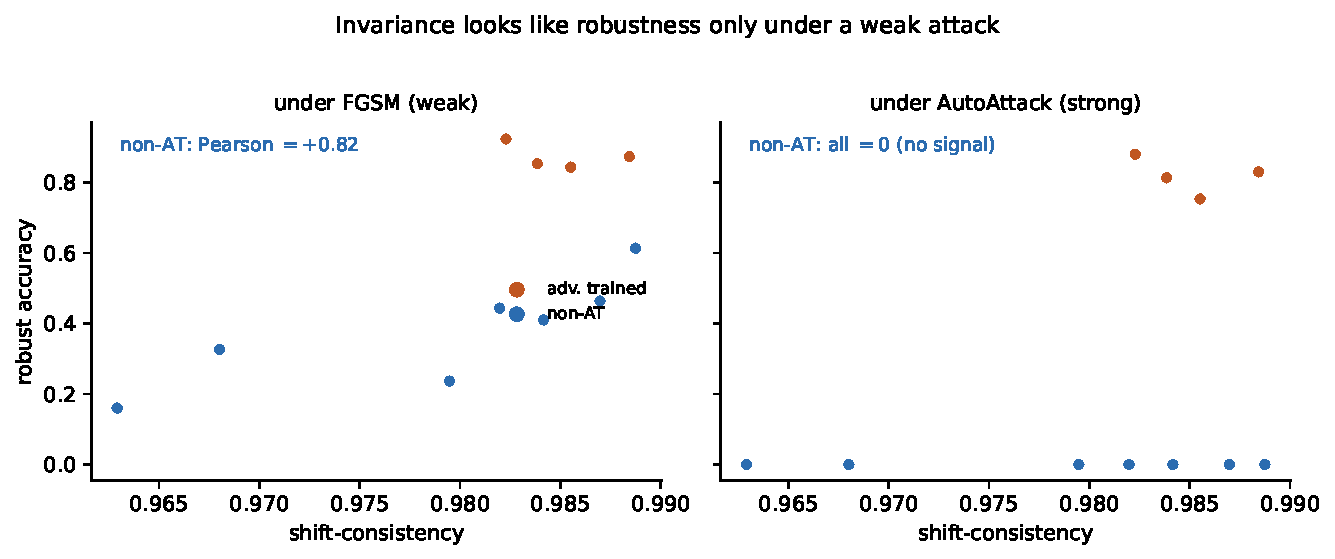
\includegraphics[width=\linewidth]{figures/fig3_weakattack.pdf}\\[0.2em]
      {\scriptsize\color{slate} Same encoders and budget: consistency looks predictive under FGSM (left),
      predicts nothing under AutoAttack (right).}
    \end{column}
  \end{columns}
  \vspace{0.1em}
  {\footnotesize We find the ``invariance helps'' correlation is a weak-attack artifact; no ``helps''
  paper had applied a parameter-free strong attack.}
  \note{Say: is the helps effect real? We rerun that exact regime, weak attacks on undefended models, and
  add AutoAttack. Under FGSM the ordering shows up. Under AutoAttack the models are all non-robust and the
  ordering is gone. So the helps effect is a weak-attack artifact, and nobody in that line had run a
  strong attack.}
\end{frame}

%========================= EXPERIMENTS: PER IMAGE =============================
\begin{frame}{Per image, where training cannot confound}{}
  \vspace{0.2em}
  \begin{columns}[T]
    \begin{column}{0.5\textwidth}
      \begin{itemize}\footnotesize\itemsep4pt
        \item On sixteen frozen CLIP encoders shift-consistency is \emph{saturated}, $0.963$--$0.988$,
          robust or not, so it cannot rank them.
        \item Within one robust encoder, image by image, $\etaL$ orders each image's radius at Spearman
          $+0.74$ to $+0.96$; per-image consistency from $+0.37$ down to about zero. Inside one encoder,
          training is not the confound.
      \end{itemize}
    \end{column}
    \begin{column}{0.48\textwidth}
      \centering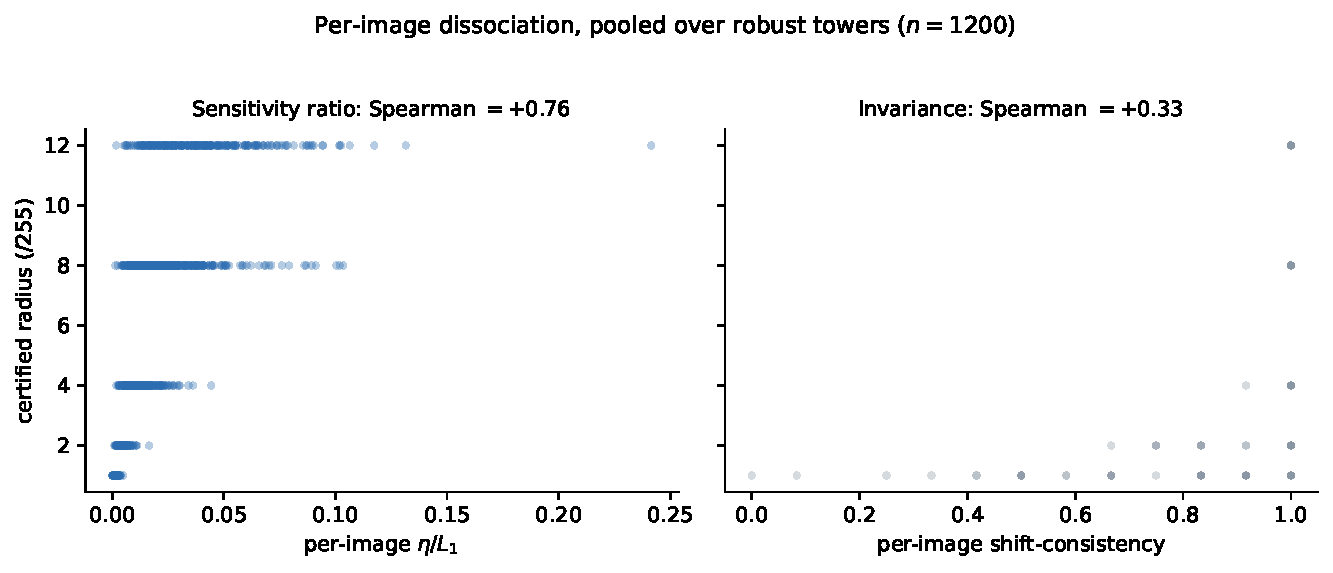
\includegraphics[width=0.98\linewidth]{figures/fig2_perimage.pdf}\\[0.2em]
      {\scriptsize\color{slate} Pooled over robust encoders ($n{=}1200$): $\etaL$ (left) orders the
      per-image radius; consistency (right) does not.}
    \end{column}
  \end{columns}
  \note{Say: on modern encoders the invariance metric is saturated, it sits near 0.98 for everyone, so it
  cannot rank. The clean test is per image inside one encoder, where training cannot confound: there the
  ratio orders each image's radius strongly, and consistency does not.}
\end{frame}

%========================= ANISOTROPY =========================================
\begin{frame}{Ranking already-robust models: the gradient's shape}{}
  \vspace{0.2em}
  \begin{columns}[T]
    \begin{column}{0.5\textwidth}
      \begin{itemize}\footnotesize\itemsep3pt
        \item Among robust models $\etaL$ no longer orders them. Add the gradient's anisotropy
          $A=\lVert\nabla M\rVert_1/\lVert\nabla M\rVert_2\in[1,\sqrt d]$: an $\ell_\infty$ attack wastes
          budget on a concentrated gradient, exploits a spread one.
        \item Over thirty RobustBench CIFAR-10 models, lower $A$ is more robust: Spearman $-0.79$
          ($-0.77$ controlling clean accuracy). Replicates on MNIST/Fashion.
        \item \key{Proposed mechanism} (not a theorem): a spread-over-dimensions deficit
          $\;r\approx(\eta/L_1)/(1+CA)$, checked on a controlled model and thirty real ones.
      \end{itemize}
    \end{column}
    \begin{column}{0.48\textwidth}
      \centering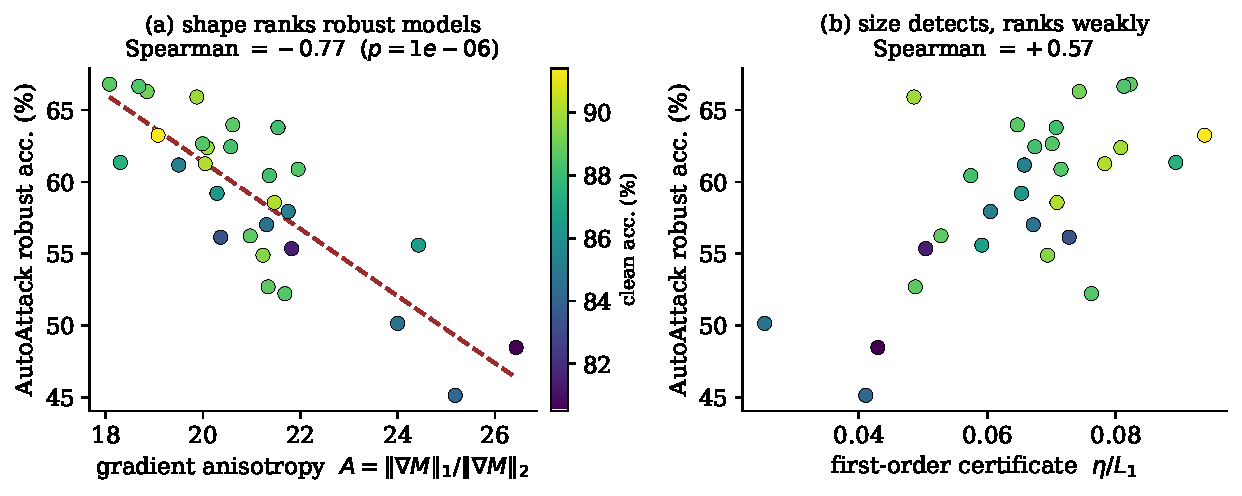
\includegraphics[width=0.99\linewidth]{figures/robustbench_aniso.pdf}\\[0.2em]
      {\scriptsize\color{slate} 30 RobustBench models. (a) the shape $A$ ranks robustness; (b) the size
      $\etaL$ detects but ranks weakly.}
    \end{column}
  \end{columns}
  \note{Say: among robust models the ratio no longer separates them. What does is the shape of the
  gradient: an L1 over L2 anisotropy. An infinity-norm attack wastes budget on a concentrated gradient and
  exploits a spread one, so lower anisotropy is more robust. On thirty RobustBench models the correlation
  is minus 0.79, surviving a clean-accuracy control. We propose a spread-over-dimensions deficit as the
  mechanism, and verify it, but we call it a proposed mechanism, not a theorem.}
\end{frame}

%========================= RESULTS TABLE ======================================
\begin{frame}{The results across settings}{}
  \vspace{0.3em}
  \centering\small
  \begin{tabular}{llccc}
    \toprule
    setting & attack / metric & \good{$\etaL$} & \bad{consist.} & shape $A$\\
    \midrule
    CIFAR-10 (standard) & min-norm radius & $+0.998$ & $-0.33$\,n.s. & ---\\
    MNIST / Fashion (AT sweep) & AutoAttack $\ell_\infty$ & predicts & n.s. & $-0.61$ to $-0.89$\\
    PreActResNet-18 (adv.\ tr.) & AutoAttack $\ell_\infty$ & $+0.91$ & $-0.81$ & ---\\
    ImageNet-100 (adv.\ tr.) & AutoAttack $\ell_\infty$ & $+0.90$ & $-0.87$ & ---\\
    16 CLIP encoders (per image) & min-norm radius & $+0.74$ to $+0.96$ & $\approx0$ & ---\\
    30 RobustBench models & AutoAttack $\ell_\infty$ & detects & --- & $-0.77$\\
    \bottomrule
  \end{tabular}
  \vspace{0.4em}
  {\scriptsize\color{slate} Pearson or Spearman as appropriate; $\etaL$ is threat-matched (dual norm
  matched to the attack). \key{n.s.}\ = not statistically significant; \key{$\approx0$} = does not order
  the radius; \key{---} = not applicable or not measured. The shape $A$ is computed only where we
  \emph{rank already-robust} models (RobustBench, and the MNIST/Fashion training-strength sweep), so it is
  blank in the other rows; shift-consistency was not measured for the downloaded RobustBench models. Every
  number reproduces from the released code and result files.}
  \note{Say: one table. The threat-matched ratio orders robustness in every setting; shift-consistency
  does not, and near zero means it does not order the radius; the shape term ranks the already-robust
  models, so it only appears in the rows where we rank robust models. The blanks are cases we did not
  measure that quantity, for example we did not compute shift-consistency for the downloaded RobustBench
  models.}
\end{frame}

%========================= LIMITATIONS ========================================
\begin{frame}{Where it breaks}{}
  \vspace{0.4em}
  \begin{itemize}\footnotesize\itemsep6pt
    \item \key{The ratio is not a trainable target.} It is scale-free, so its direct maximizer is the
      constant classifier. It is a diagnostic, not a loss.
    \item \key{The shape law needs range.} On low-dimensional data the anisotropy is compressed and does
      not rank until a training-strength sweep widens the range; the clean cross-model evidence is
      RobustBench.
    \item \key{The deficit is proposed, not proven.} We verify it on a controlled model and thirty real
      ones, but it is not a network-level theorem.
    \item \key{Text-modality robustness stays narrow.} On CLIP the worst case over a small paraphrase set
      is too mild to form a second adversarial axis.
  \end{itemize}
  \note{Say: where it breaks. The ratio cannot be trained toward, it is scale-free and its maximizer is
  trivial. The shape law needs a wide robustness range to show. The deficit is a proposed mechanism, not
  a proof. And on text the worst case over a small paraphrase set is too weak to be a real adversarial
  axis. I am stating these on purpose.}
\end{frame}

%========================= NEW VS PRIOR (placeholder table, verified) =========
\begin{frame}{Proposed contributions, and existing results}{Verified against the primary sources}
  \vspace{0.2em}
  \centering\scriptsize
  \begin{tabular}{p{5.8cm}p{5.8cm}}
    \toprule
    \textbf{\color{good}Proposed contribution} & \textbf{\color{slate}Existing result we use or refine}\\
    \midrule
    Consistency does not order robustness while threat-matched $\etaL$ does, across model families &
    The certificate $r\ge M/\lVert\nabla M\rVert$: \tb{Hein \& Andriushchenko 2017; Tsuzuku et al.\ 2018}\\
    The powered per-image dissociation within one frozen encoder (training cannot confound) &
    Attack-free radius estimates: CLEVER \tb{(Weng et al.\ 2018)}\\
    The ``invariance helps'' effect vanishes under a parameter-free strong attack &
    That invariance and robustness are related: \tb{Ge; Kamath; Saha; Wang}\\
    The upper arm of the bracket, $r\le\eta/\alpha$, with an explicit condition number $\kappa$ &
    The DC-collapse / margin mechanism: \tb{Ge et al.\ 2021}\\
    Anisotropy $\lVert\nabla M\rVert_1/\lVert\nabla M\rVert_2$ ranks already-robust models &
    Certified radii via smoothing: \tb{Cohen et al.\ 2019}\\
    The effective-dimension deficit as its (proposed) mechanism &
    Gradient-dimension and curvature views: \tb{Simon-Gabriel 2019; Moosavi 2019}\\
    Saturation of shift-consistency on modern encoders, and its textual analogue &
    Participation-ratio of the input gradient (overfitting detection): \tb{2025}\\
    The margin--sensitivity sign-flip under adversarial training &
    AutoAttack as the arbiter: \tb{Croce \& Hein 2020}; margin consistency in robust models: \tb{Ngnawe 2024}\\
    \bottomrule
  \end{tabular}
  \note{Say: to be explicit about the contribution. On the left, the proposed contributions: the
  dissociation, the powered per-image version, the weak-attack result, the upper bound of the bracket,
  the anisotropy ranking, its mechanism, the saturation, and the sign-flip. On the right, the existing
  results we use or refine: the certificate itself, CLEVER, the fact these are related, the DC mechanism,
  randomized smoothing, the dimension and curvature views, the participation ratio, AutoAttack, and
  Ngnawe's margin consistency.}
\end{frame}

%========================= CONCLUSION =========================================
\begin{frame}{Summary and directions}{}
  \vspace{0.4em}
  \begin{itemize}\footnotesize\itemsep5pt
    \item Shift-consistency, the metric this literature tracks, does not order adversarial robustness, and
      the ``invariance helps'' effect vanishes under a strong attack.
    \item A threat-matched, scale-free margin-to-Lipschitz ratio, which we complete to a two-sided
      bracket, orders robustness from small classifiers to frozen CLIP encoders.
    \item To rank already-robust models, the shape of the gradient (its anisotropy) matters, through a
      spread-over-dimensions deficit.
  \end{itemize}
  \vspace{0.4em}
  {\footnotesize\color{slate}\textbf{Next directions:} beyond $\ell_\infty$; the rich-regime
  optimization / implicit-bias question; a genuine text-adversarial axis; scaling the anisotropy study
  beyond RobustBench.}
  \note{Say: to summarize. Consistency does not order robustness and the helps effect is a weak-attack
  artifact. A threat-matched, scale-free margin ratio, with a two-sided bracket, orders robustness across
  families. And ranking robust models needs the gradient's shape. Next directions: other norms, the
  optimization question, a real text attack, and scaling the anisotropy study.}
\end{frame}

%========================= QUESTIONS FOR MAHA =================================
\begin{frame}{Where your input would help most}{}
  \vspace{0.3em}
  \begin{itemize}\footnotesize\itemsep5pt
    \item \key{Positioning as a certificate.} $\etaL$ is a Lipschitz--margin certificate we complete to a
      two-sided bracket. Given your work on robustness certificates, is the bracket a meaningful addition,
      or is it subsumed by existing certified methods (randomized smoothing, Lipschitz certification)?
      What is the cleanest framing of ``certificate vs diagnostic''?
    \item \key{The kernel / lazy-regime theory.} Our lazy-regime result treats orbit-averaging as a
      projection in the tangent-kernel space. Given your deep-net-to-kernel-machine work, is this the
      right lens, and where are the pitfalls (e.g.\ the bare-ReLU NTK is not Lipschitz)?
    \item \key{Weakest parts / experiments.} Which pieces look weakest to you, the small robust-encoder
      panel, the range-dependence of the anisotropy law, the proposed-not-proven deficit, and which
      experiments would you rerun or design differently?
    \item \key{Literature and framing.} Are we missing work at the certified-robustness $\times$
      invariance intersection? And is the dissociation, or the anisotropy law, the stronger headline?
  \end{itemize}
  \note{Say: this is where your input would help most. First, positioning: eta over L is a certificate,
  and we add a two-sided bracket; given your certificate work, is that a real addition or subsumed by
  smoothing and Lipschitz methods, and how should we frame certificate versus diagnostic. Second, the
  kernel theory: our lazy-regime result is a projection in the tangent kernel space, is that the right
  lens given your kernel work. Third, which parts are weakest and what would you rerun. Fourth, missing
  literature, and which result should headline.}
\end{frame}

\end{document}
